%; whizzy document
% latex beamer presentation.
% platex, latex-beamer でコンパイルすることを想定。 

%     Tokyo Debian Meeting resources
%     Copyright (C) 2007 Junichi Uekawa

%     This program is free software; you can redistribute it and/or modify
%     it under the terms of the GNU General Public License as published by
%     the Free Software Foundation; either version 2 of the License, or
%     (at your option) any later version.

%     This program is distributed in the hope that it will be useful,
%     but WITHOUT ANY WARRANTY; without even the implied warranty of
%     MERCHANTABILITY or FITNESS FOR A PARTICULAR PURPOSE.  See the
%     GNU General Public License for more details.

%     You should have received a copy of the GNU General Public License
%     along with this program; if not, write to the Free Software
%     Foundation, Inc., 51 Franklin St, Fifth Floor, Boston, MA  02110-1301 USA

% 実行順番
% sudo  ~/bin/usb-macbook-ir.c &
% real presentation (shell-command (concat "DISPLAY=:0.1 xpdf -fullscreen " (replace-regexp-in-string "tex$" "pdf"(buffer-file-name)) "&"))
% DISPLAY=:0.1 xpdf -fullscreen 

\documentclass[cjk,dvipdfmx]{beamer}
\usetheme{Warsaw}
%  preview (shell-command (concat "xpdf " (replace-regexp-in-string "tex$" "pdf"(buffer-file-name)) "&"))
%  presentation (shell-command (concat "xpdf -fullscreen " (replace-regexp-in-string "tex$" "pdf"(buffer-file-name)) "&"))

%http://www.naney.org/diki/dk/hyperref.html
%日本語EUC系環境の時
\AtBeginDvi{\special{pdf:tounicode EUC-UCS2}}
%シフトJIS系環境の時
%\AtBeginDvi{\special{pdf:tounicode 90ms-RKSJ-UCS2}}

\title{東京エリア Debian 勉強会}
\subtitle{資料}
\author{上川 純一 dancer@debian.org\\IRC nick: dancerj}
\date{2007年1月20日}
\logo{
\includegraphics[width=8cm]{image200607/openlogo-light.eps}}

% 三択問題用
\newcounter{santakucounter}
\newcommand{\santaku}[5]{%
\addtocounter{santakucounter}{1}
\frame{\frametitle{問題\arabic{santakucounter}. #1}
%問題\arabic{santakucounter}. #1
\begin{minipage}[t]{0.7\hsize}
 \begin{itemize}
 \item  A #2\\
 \item  B #3\\
 \item  C #4\\
 \end{itemize}
\end{minipage}
}
\frame{\frametitle{問題\arabic{santakucounter}. #1}
%問題\arabic{santakucounter}. #1
\begin{minipage}[t]{0.7\hsize}
\begin{itemize}
\item  A #2\\
\item  B #3\\
\item  C #4\\
\end{itemize}
\end{minipage}
\begin{minipage}[t]{0.2\hsize}
答えは:

\vspace{1cm}

{\huge \hspace{1cm}#5}
\end{minipage}}
}


\begin{document}
\frame{\titlepage{}}

\section{Intro}

\begin{frame}
 \frametitle{本日のagenda}
\begin{minipage}[t]{0.4\hsize}
  \begin{itemize}
  \item 注意事項
	\begin{itemize}
	 \item 飲食禁止
	 \item 政治/宗教/営利活動禁止
	\end{itemize}
  \item 最近事情
  \item 事前課題紹介
  \item quiz
 \end{itemize}
\end{minipage} 
\begin{minipage}[t]{0.4\hsize}
 \begin{itemize}
  \item apt-torrent
  \item kvm
  \item 2007年のDebian勉強会を計画する
  \item quilt
  \item 今後のイベント
 \end{itemize}
\end{minipage}
\end{frame}

\section{最近のDebian関連のミーティング報告}

\begin{frame}{最近のDebian関連ミーティング報告}
 \begin{itemize}
  \item Debian勉強会
 \end{itemize}
\end{frame}

\begin{frame}
 \frametitle{2006年12月のagenda}
\begin{minipage}[t]{0.4\hsize}
  \begin{itemize}
  \item 注意事項
	\begin{itemize}
	 \item 飲食禁止
	 \item 政治/宗教/営利活動禁止
	\end{itemize}
  \item 最近事情
  \item 事前課題紹介
  \item quiz
 \end{itemize}
\end{minipage} 
\begin{minipage}[t]{0.4\hsize}
 \begin{itemize}
  \item Bug Squashing Partyについて
  \item 来年の Debian 勉強会を設計する
 \end{itemize}
\end{minipage}
\end{frame}

\section{事前課題の声}
\begin{frame}

 今回の事前課題は
「今後、勉強会につかう施設を提案してください」と「2007年の勉強会の各
 月のアジェンダを提案してください」
 というタイトルで200-800文字程度の文章を書いてください。というものでした。
 その課題に対して下記の内容を提出いただきました。
\end{frame}


\subsection{Ishihara さん}

\begin{frame}{「今後、勉強会につかう施設を提案してください」}

角筈地域センター
公共の施設が安くて便利そうな気がします。
ただ、電源やLANとかそういう設備が厳しいのかもしれません。
個人的にはこういうところでの勉強会もやってみたいかも。
\end{frame}

\begin{frame}{「2007年の勉強会の各月のアジェンダを提案してください」}
\small

・古いPC復活大作戦
\begin{enumerate}
 \item 古いマシンをDebianで復活させる:    古いマシン独特の問題
 \item デスクトップ機にしてみる:  Xつかうよ or Xつかわないよ
 \item サーバにしてみる:      セキュリティの問題
\end{enumerate}
みたいな感じで、ちょっと型落ちなマシンを復活させる、という実践的?な企画が
あってもいいかなぁと思います。
1年でサーバマシンが立てられるよ、セキュリティもちゃんと配慮できるよ、みたいな企画ですね。

あとは、Debianに関係する英語を読んで見ましょう企画とか。

・vs 英語
\begin{enumerate}
 \item Debianの英語サイトを読んでみよう:
     キーワードの見つけ方、
     英語の辞書の使い方、
     どのドキュメントを読めばいいの?
\end{enumerate}
やっぱりネックとなるのは英語なメッセージやドキュメントだと思います。
ググれ、と突き放すのもひとつの勉強法なんですけど、
ちょっとでも読み方がわかると、敷居が低くなるんじゃないのかなぁと思うのですが。
どうなんでしょうか?
\end{frame}


\subsection{小林儀匡}

\begin{frame}{『今後、勉強会につかう施設を提案してください』}

\tiny

これまで何回か「大学は利用できないのか」という話があったこともあり、
大学所属のメンバーとして、勉強会に使える施設が大学内にないか検討してみました。

まず、情報教育のための施設である情報教育棟
については、『情報教育棟 
会議室・セミナー室利用申込』
の利
用規定第2条(1)に、教職員が学部、専攻(系)、学科、部会、センター、委員会、
事務部が主宰する会合、とありました。
学生がサークルのようなものの集まりとして使用するような使い方はできないようです。
まぁ、
得体の知れない人間にコンピュータやネットワークを自由に利用されても困りますので、
仕方がないでしょうか。

次に、
サークルなどで使われている東京大学駒場コミュニケーション・プラザも検討してみました。
こちらの利用規則には次のようにあります。

(中略)

例外的に適当と認められるために何をすればよいのかよくわかりませんが、
それなりの手続きを経なければいけないようです。

大学という場はオープンで結構使いやすいかと思われがちですが、
オープンすぎて勝手に使われると問題になるので案外色々と制限 (「主催者が教職員」とか「構成員が学内の人間」とか) がかかっていることが多いです。
昨年11月の大阪電気通信大学での勉強会のように教員が誘致してくださったりする場合はやりやすいでしょうが、
そうでない場合はなかなか使いにくい場ではないでしょうか。
まだまだ探す余地はあると思うのでもう少し粘ろうかと思いますが……。
\end{frame}

\begin{frame}{『2007年の勉強会の各月のアジェンダを提案してください』}

{\tiny
\begin{description}
 \item[2月] 「今年、私はDebianにこのように関わろうと思います/○○を成し遂げます!!」宣言大会
 \item[3月] Debian etchリリース記念インストール大会
 \item[4月] Debian lennyに向けて日本語圏でやっておきたい事項のリストアップ
 \item[5月] Debianを使っていて思う「このようなフリーなアプリケーションが足りない」
 \item[6月] Debian Conference 7現地報告
 \item[7月] Debian Conference 7報告
 \item[8月] Debianでのウェブアプリケーションのあれこれ
 \item[9月] Debianでのグラフィックアプリケーションのあれこれ
 \item[10月] Debianの派生ディストリビューションのあれこれ
 \item[11月] Debianと私
 \item[12月] 「今年、私はDebianに関して○○を成し遂げました/成し遂げられませんでした」報告・反省大会
\end{description}
}
\end{frame}

\subsection{前田 耕平さん}

\begin{frame}{「今後、勉強会につかう施設を提案してください」}

二箇所提案します。

\begin{enumerate}
 \item  晴海区民館:
 晴海トリトンにあります。ちょっと高いのが難点です。

 \item 月島区民館
 宴会を月島のお好み焼きや、もんじゃ焼きに絞る場合はこちらの方が良いかも。
	(ただ、月島の店は閉店が早いです。23時にしまっちゃいます)
\end{enumerate}

あまり現実的ではありませんが、私の住んでいるマンションの共有施設、という手もあります。
利用料は安いのですが(300円or500円/1時間)、交通の便があまりよくありません。
あと、近くに飲み屋どころか、飲食店がほとんどありません。(あっても23時で閉店なので)
だからといってウチで飲み会、というのは困るので…。

\end{frame}

\begin{frame}{「2007年の勉強会の各月のアジェンダを提案してください」}

バッティングしそうなのもあるので、ネタだけ列挙します。

{\small
\begin{enumerate}
 \item Debianでだってできる3Dデスクトップs 裏番組(Vista)をぶっ潰せ!
 \item Etchリリース(仮)を祝って、Sarge→Etchのアップグレード苦労話
 \item 新入生・新入社員をDebianユーザにする企て
 \item 打ち上げ花火でDebianのグルグルを実現できるか(趣旨違いますね)
 \item Debian勉強会@Linux World又はLC(って今年も開催するのか?)
 \item 他のユーザ会とのコラボ(特にターゲットは無し)
\end{enumerate}
}

\end{frame}

\subsection{岩松 信洋}


\begin{frame}{「今後、勉強会につかう施設を提案してください」}

自分の勤務地の最寄り駅である国分寺駅近辺の施設を調べてみました。
いいところがありませんでした。
	
\end{frame}

\begin{frame}{「2007年の勉強会の各月のアジェンダを提案してください」}
 \tiny
\begin{itemize}
 \item	 2月 パッケージ依存関係を図にして印刷してみる:
		apt-cache dotty で出力された dotty ファイルをプリントアウト
		して満足する。
		
 \item	 3月 東京青少年オリンピックセンター 合宿 and OSC 2007 spring:
		合宿をする。
		OSC に参加して本を売る。

 \item	 4月 dbs を調べてみる:
		あまりメジャーではない dbs について熱く語る。

 \item	 5月 defoma を解析して、熱く語る。:
		山根さんが defoma を解析して、熱く語る。

 \item	 6月 debconf and OSC DO 2007:
		debconf組がエジンバラに行っている間、残った人はみんな
		北海道で合宿。

 \item	 7月 apt-xxx を調べる:
		実はみんなが知らない apt-xxx があるのではないか?
		調べて熱く語る。

 \item	 8月  ラインセンスを調べる  and コミケ:
		Debian パッケージの ライセンスを全て調べてみる。
		コミケをがんばる。

 \item	 9月 OSC 2007 Tokyo Fall に参加:
		OSCに参加する。

 \item	 10月 Debian で 動画再生環境を作ってみる:
		main セクションだけで動画再生環境を作ったらどうなるか、調べる。

 \item 	 11月 KOF に参加:
		KOFに参加して、○○さん実家に泊まる。

 \item	 12月 反省会 and コミケ:
		コミケをがんばる。
		反省会もちゃんとする。
		温泉合宿を決行する。
\end{itemize}
\end{frame}

\subsection{北原さん}


\begin{frame}{今後、勉強会につかう施設を提案してください}
\tiny

  現在と同じような勉強会(曜日・時間・人数・プロ
ジェクター等の施設)が出来る施設を探してみました。
現在利用している施設の使用料がわからないので、参加
費と人数、資料代等を適当に勘案して、1万円以下を条
件としました。

  そうすると、民間の物件はほとんど不可能なので、
公共の施設となりますが、区の施設では利用者の制限が
厳しい(半数が区民である必要がある等)ので都の施設
を調べてみました。

  以前の勉強会で話題に挙がった、東京体育館、同じ
団体で管理している東京武道館・駒沢オリンピック公園
総合運動場・東京辰己国際水泳場(全て会議室あり)を
除くとあまり良いのは見つかりませんでした。

  その中でも「東京スポーツ文化館・BumB」が、利用
条件が緩く、2,625円からで利用できそうです(場所は夢の
島)。 勉強会に「男女平等の推進に関する」テーマが
盛り込めれば、「東京ウィメンズプラザ」(場所は神宮
前)が利用できるかも?(笑)(3,300円から)

  夜でなくても良ければ「東京国際ユースホステル」
の研修室が利用でるかも?(飯田橋の駅側、3,000円)

  あと、利用方法が調べきれていませんが、清澄庭園
・蘆花恒春園でも集会所が借りられるようですが、ちょ
いと勉強会とは雰囲気が違うような気がする。

  国関係も調べようと試みましたが、まったく引っか
かりませんでした。(調べ方が悪かったかも)

  あと、「東京スポーツ文化館・BumB」は宿泊施設が
あって最大251人(定員)泊まれます。 DebConfの検討
対象にはなりませんかね?


\end{frame}

\subsection{小室 文さん}

\begin{frame}{今後、勉強会につかう施設を提案してください}
\small

練馬区在住なので、練馬区施設関連を中心に探しました。

貫井地区区民館
最寄:中村橋駅(西武池袋線)徒歩5分
1時間400円

光が丘地区区民館

最寄:光が丘駅(大江戸線)
1時間:500円

石神井公園区民交流センター
最寄:石神井公園(西武池袋線)
会議室(1):1200円

練馬女性センター
最寄:石神井公園駅(西武池袋線)
第1研修室:1400円

後は学校開放というのをしていて、会議室がある小学校が夜間貸し出しをしてい
る所があるようです。
夜間は18時から21時で、大体600円ぐらいです。

練馬まで来てくれるかっというのが最大の問題ですね・・・

\end{frame}

\begin{frame}{2007年の勉強会の各月のagenda}

暗号化とは!?とか・・自分で調べたら分かるよなぁという事もただあるので、
なかなか思いつかないですね。「これだけは絶対やってはいけない操作」とかど
うでしょう。後は個人的にDebian policyは勉強したいと思います。ちゃんとし
た回答になっていなくてすいません・・・

\end{frame}


\section{DWNQuiz}
%% debianmeetingresume200701.texから以下コピー

\subsection{2006年42号}
\url{http://www.debian.org/News/weekly/2006/42/}
にある2006年12月26日版です。

\santaku
{Linux Conference Australia で開催される Debian 関係のイベントは今回で何回目か}
{1}
{3}
{6}
{C}

\santaku
{最近急上昇してDebian内で3位人気のアーキテクチャになったアーキテクチャは?}
{ARM}
{PPC}
{AMD64}
{A}

\santaku
{etchがフリーズされたのはいつ?}
{11/11}
{12/11}
{12/24}
{B}

\santaku
{Debian のインストール CD イメージはどれくらいの頻度で更新されているか?}
{毎日}
{毎メジャーリリース}
{毎マイナーリリース}
{A}


\begin{frame}{apt-torrent}
 
岩松さん
\end{frame}


\section{kvm}

\begin{frame}[containsverbatim]{インストール方法}
2.6.20 以降の最新のカーネルをインストール

\begin{verbatim}
apt-get install kvm
\end{verbatim}
VT 命令を BIOS で enable
\end{frame}

\begin{frame}[containsverbatim]{利用方法}
\begin{verbatim}
$ qemu-img create -f qcow hda 10G
$ sudo chown dancer:dancer /dev/kvm
$ kvm -hda hda -cdrom /home/iso/RHEL4-U4-i386-AS-disc1.iso
   -boot d -m 512 -monitor stdio


$ kvm -hda hda  -boot c -m 512 -monitor stdio -localtime  \
 -redir tcp:2222::22
\end{verbatim}
\end{frame}

\begin{frame}{実行画面}
\begin{minipage}{0.4\hsize}
 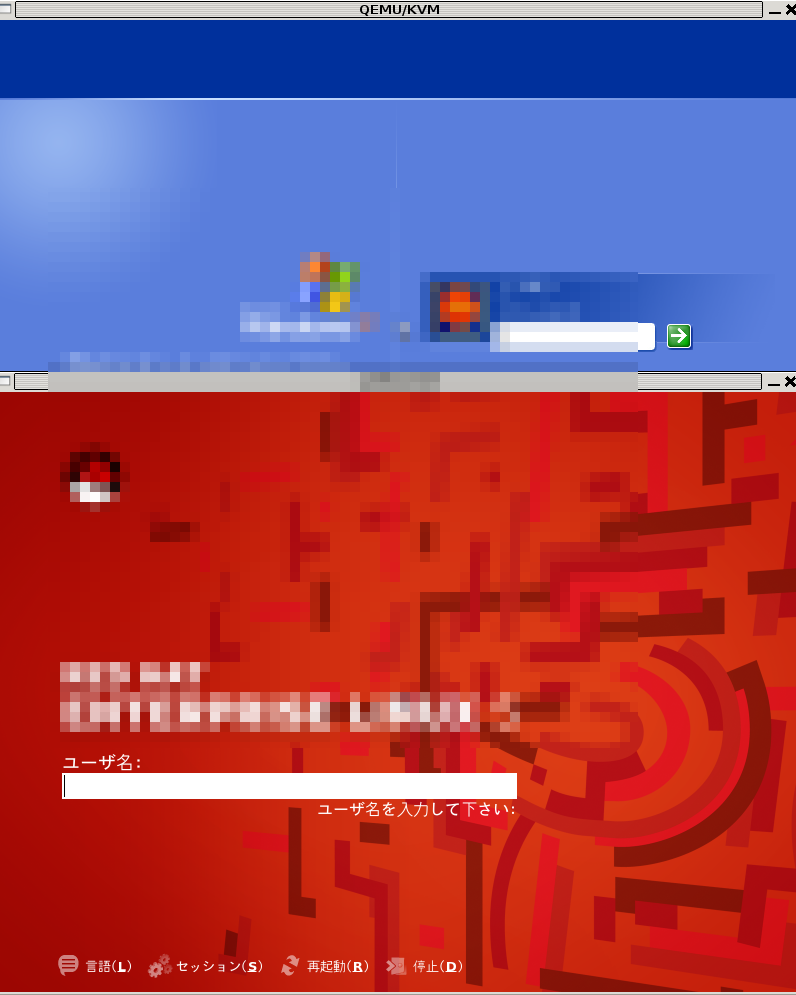
\includegraphics[width=0.9\hsize]{image200701/kvm.png}
\end{minipage}
\begin{minipage}{0.5\hsize}
無事に動作します。
\end{minipage}
\end{frame}

\section{2007年度計画}

\begin{frame}

 19:55 まで、計画立案

\end{frame}

\begin{frame}{背景}
\tiny
Debianが今提供している付加価値は「\underline{\hspace{8cm}}」です。
2007年に発生しそうな外部的なイベントは次の項目です
\begin{itemize}
 \item Windows: (\underline{\hspace{8cm}})
 \item Mac OS X:(\underline{\hspace{8cm}})
 \item 他のディストリビューション: (\underline{\hspace{8cm}})
 \item ハードウェア: (\underline{\hspace{8cm}})
 \item ユーザの期待: (\underline{\hspace{8cm}})
 \item (\underline{\hspace{8cm}})
\end{itemize}

この状況を踏まえて Debian 勉強会が成し遂げるべきことは

「\underline{\hspace{8cm}}」です。

これらを踏まえて2007年のDebian 勉強会のテーマは

「\underline{\hspace{8cm}}」

とします。
\end{frame}

\begin{frame}
\tiny
 
ここで、2007年の12ヶ月分のアジェンダを作成します。

\begin{description}
 \item[1月] 新年会(\underline{\hspace{8cm}})
 \item[2月] (\underline{\hspace{8cm}})
 \item[3月] OSC? (\underline{\hspace{8cm}})
 \item[4月] OSC-Do? (\underline{\hspace{8cm}})
 \item[5月] Debconfプレゼンリハーサル (\underline{\hspace{8cm}})
 \item[6月] Debconfエジンバラ開催 (\underline{\hspace{8cm}})
 \item[7月] Debconf参加報告会(\underline{\hspace{8cm}})
 \item[8月] Debian 14周年 (\underline{\hspace{8cm}})
 \item[9月] (\underline{\hspace{8cm}})
 \item[10月] OSC-Fall? (\underline{\hspace{8cm}})
 \item[11月] KOF? (\underline{\hspace{8cm}})
 \item[12月] 忘年会(\underline{\hspace{8cm}})
\end{description}

この中で自分が主体として開催するのは
「\underline{\hspace{8cm}}」の回の内容です。

名前のブランディングとして、
通常実施の勉強会を「\underline{\hspace{8cm}}」と呼び、
大衆向けの勉強会を「\underline{\hspace{8cm}}」と呼びます。


\end{frame}

\begin{frame}{発表}
 
各チーム代表

\begin{itemize}
 \item Aチーム:20:40-
 \item Bチーム:20:45-
\end{itemize}
\end{frame}

\begin{frame}{質問}

\end{frame}



\section{今後のイベント}

\begin{frame}
 \frametitle{今後の企画}
 \begin{itemize}
  \item 2007年3月 OSC
  \item 2007年6月 Debian Conference
  \item 2007年2月 Debian 勉強会
 \end{itemize}
\end{frame}

\begin{frame}
 \frametitle{宴会会場}
 \begin{itemize}
  \item 会場:荻窪 卯(うさぎ)
  \item 時間:21:00-
  \item 集合場所: この建物 1F のところ
  \item 注意事項
	\begin{itemize}
	 \item 終電の時間をちゃんとしらべていきましょう
	\end{itemize}
 \end{itemize}
\end{frame}

\end{document}
